\documentclass[12pt]{article}
\usepackage[spanish]{babel}
\usepackage[utf8]{inputenc}
\usepackage[T1]{fontenc}
\usepackage{graphicx}
\usepackage{geometry}
\usepackage{setspace}
\usepackage[hidelinks]{hyperref}
\usepackage{float}
\usepackage{titlesec}
\usepackage{listings}
\usepackage{xcolor}
\usepackage{enumitem}
\usepackage{amsmath}

\geometry{a4paper, margin=2.5cm}

% --- Configuracion para codigo ---
\definecolor{codegreen}{rgb}{0,0.6,0}
\definecolor{codegray}{rgb}{0.5,0.5,0.5}
\definecolor{backcolour}{rgb}{0.95,0.95,0.92}

\lstset{
    backgroundcolor=\color{backcolour},   
    commentstyle=\color{codegreen},
    keywordstyle=\color{blue},
    numberstyle=\tiny\color{codegray},
    stringstyle=\color{orange},
    basicstyle=\ttfamily\footnotesize,
    breaklines=true,
    captionpos=b,
    numbers=left,
}

\begin{document}
% --- PORTADA ---
\begin{titlepage}
\begin{center}
    \includegraphics[width=0.25\textwidth]{logo-uteq.png} \\[1cm]
    {\large \textbf{UNIVERSIDAD TÉCNICA ESTATAL DE QUEVEDO}} \\[0.5cm]
    {\large \textbf{FACULTAD DE CIENCIAS DE LA COMPUTACIÓN Y DISEÑO DIGITAL}} \\[0.5cm]
    {\large \textbf{CARRERA DE SOFTWARE}} \\[2cm]
    
    \textbf{TEMA:}\\[0.5cm]
    {\Large \textbf{Evaluación Práctica Unidad II: Sistema CRUD de Materias}} \\[1cm]
    
    \textbf{ALUMNO:}\\[0.5cm]
    \textbf{CRUZ PEREZ JUSTYN KEITH} \\[1cm]

    \textbf{REPOSITORIO DE GITHUB:}\\[0.3cm]
    \href{https://github.com/keithdrox/materias-CRUZ-PEREZ}{\texttt{github.com/keithdrox/materias-CRUZ-PEREZ}} \\[1cm]
    
    \textbf{DOCENTE:}\\[0.5cm]
    ING. GUERRERO ULLOA GLEISTON CICERON\\[1cm]
    
    \textbf{MATERIA:}\\[0.5cm]
    APLICACIONES WEB - A - [5to Nivel] \\[1cm]
    
    \vfill
    Quevedo - Ecuador \\
    2026
\end{center}
\end{titlepage}

\newpage

\section{Descripción de la Práctica}

La presente práctica evaluativa de la Unidad II de la asignatura de Aplicaciones Web tiene como objetivo el diseño e implementación de un micro-sistema web seguro para la administración de las materias que ofrece la carrera de Ingeniería de Software.

El sistema fue desarrollado bajo la arquitectura Cliente-Servidor utilizando la pila tecnológica de \textbf{PHP 8.3} junto con el sistema de gestión de bases de datos relacionales \textbf{PostgreSQL}. La aplicación web asegura el acceso a la gestión de datos mediante un sistema de autenticación de administradores, protege la integridad de la base de datos con consultas SQL parametrizadas, y blinda la infraestructura contra ataques listados en el OWASP Top 10:2021.

El proyecto completo se ha estructurado de forma que sea fácilmente reproducible en cualquier entorno mediante el uso de contenedores con \textbf{Docker} y \textbf{Docker Compose}.

\section{Capturas de Pantalla}

\subsection{Login del Sistema}
\begin{figure}[H]
  \centering
  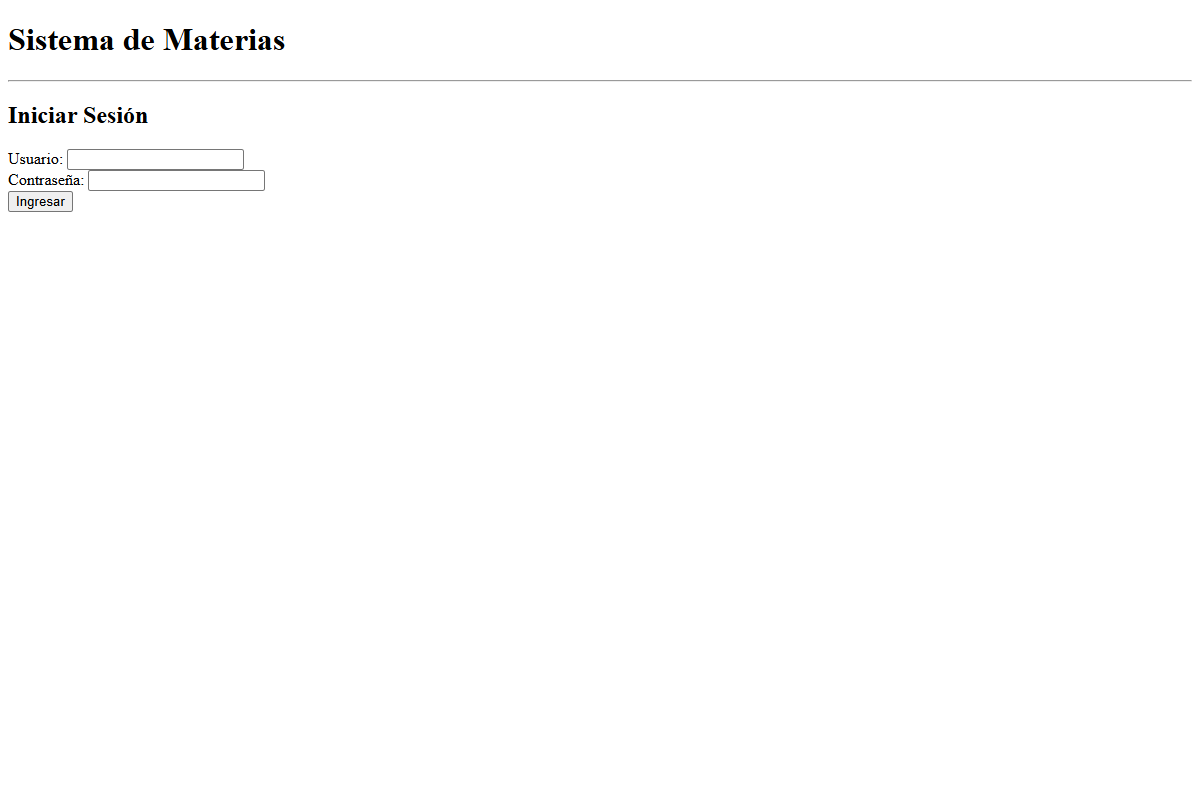
\includegraphics[width=0.8\textwidth]{capturas/01-login.png}
  \caption{Pantalla de inicio de sesión seguro.}
\end{figure}

\subsection{Listado de Materias}
\begin{figure}[H]
  \centering
  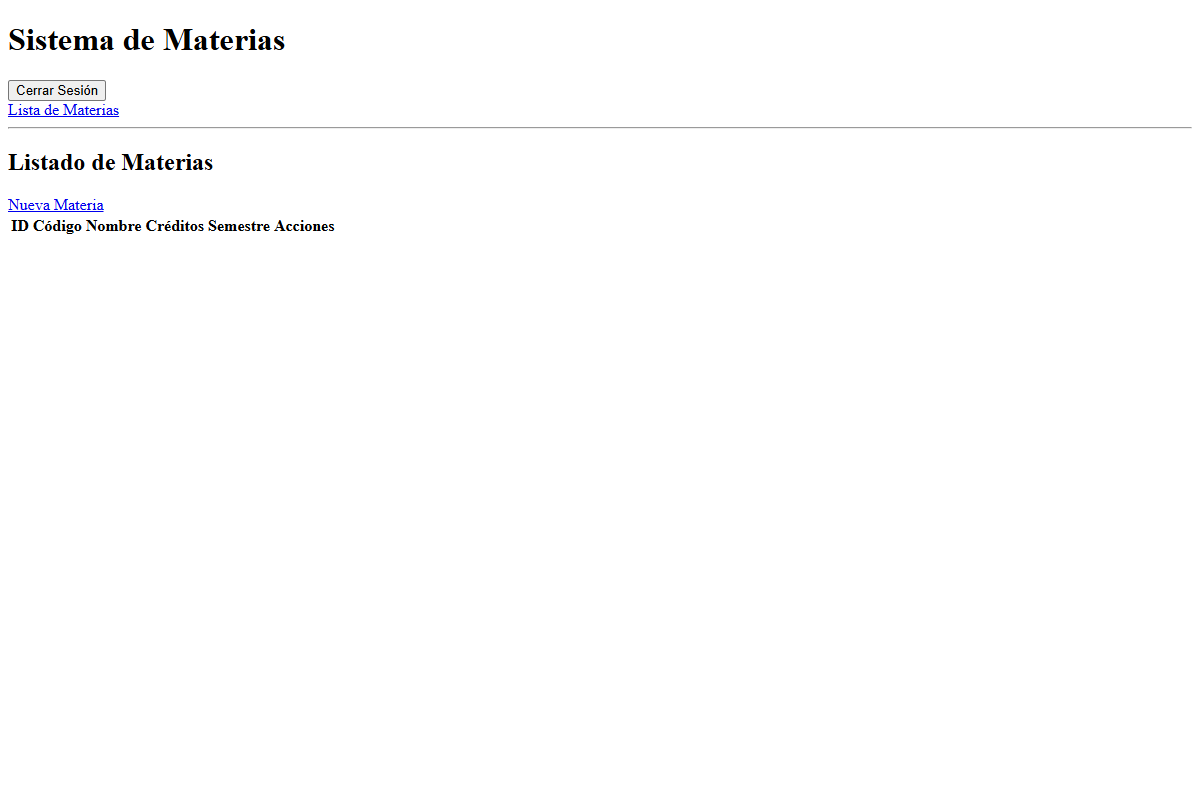
\includegraphics[width=0.8\textwidth]{capturas/02-listado.png}
  \caption{CRUD: Visualización y listado en tabla.}
\end{figure}

\subsection{Creación de Materia (Alta)}
\begin{figure}[H]
  \centering
  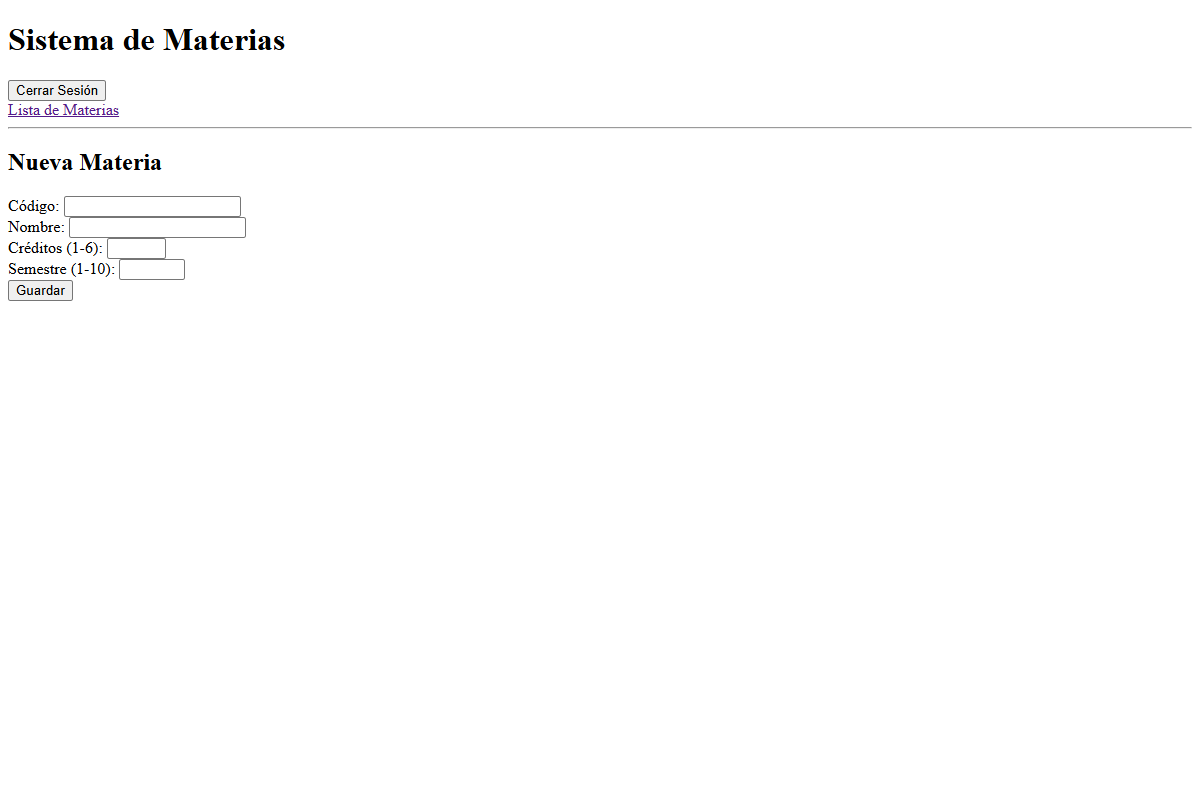
\includegraphics[width=0.8\textwidth]{capturas/03-alta.png}
  \caption{CRUD: Formulario para el alta de materias.}
\end{figure}

\subsection{Edición de Materia}
\begin{figure}[H]
  \centering
  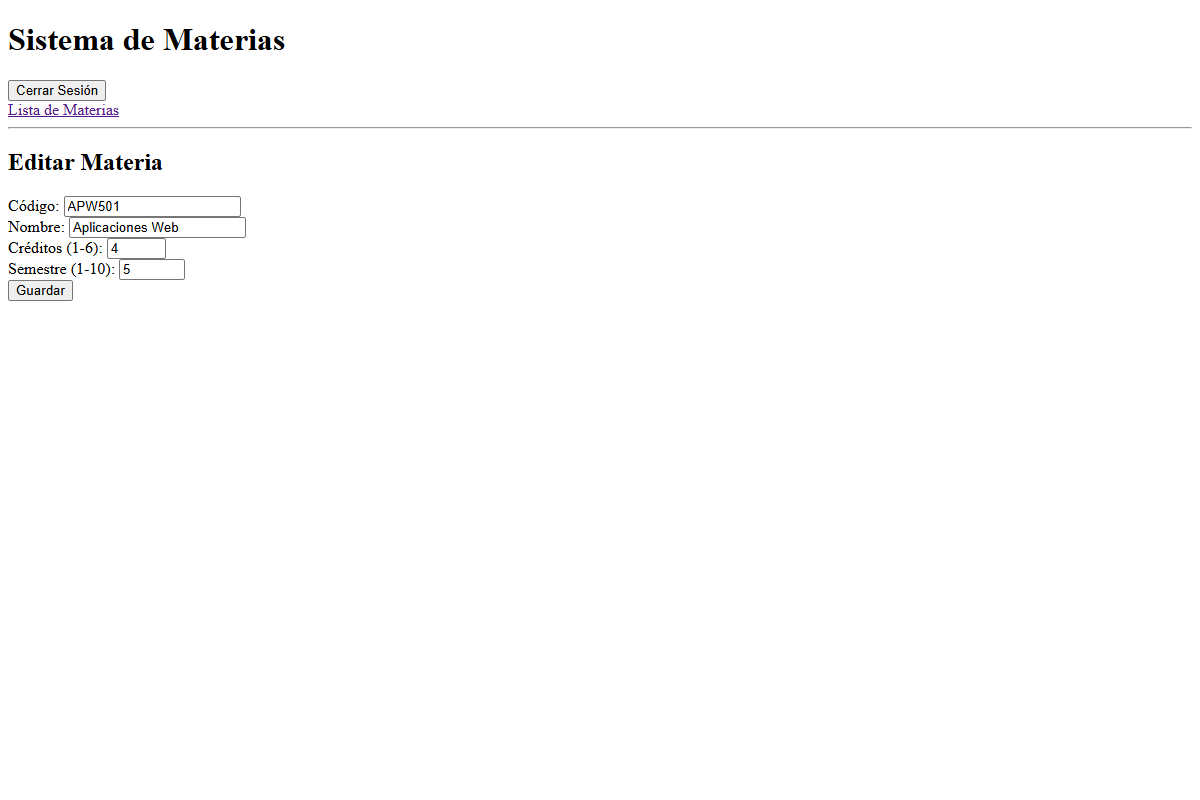
\includegraphics[width=0.8\textwidth]{capturas/04-edicion.png}
  \caption{CRUD: Formulario de actualización poblado con datos previos.}
\end{figure}

\subsection{Eliminación Lógica}
\begin{figure}[H]
  \centering
  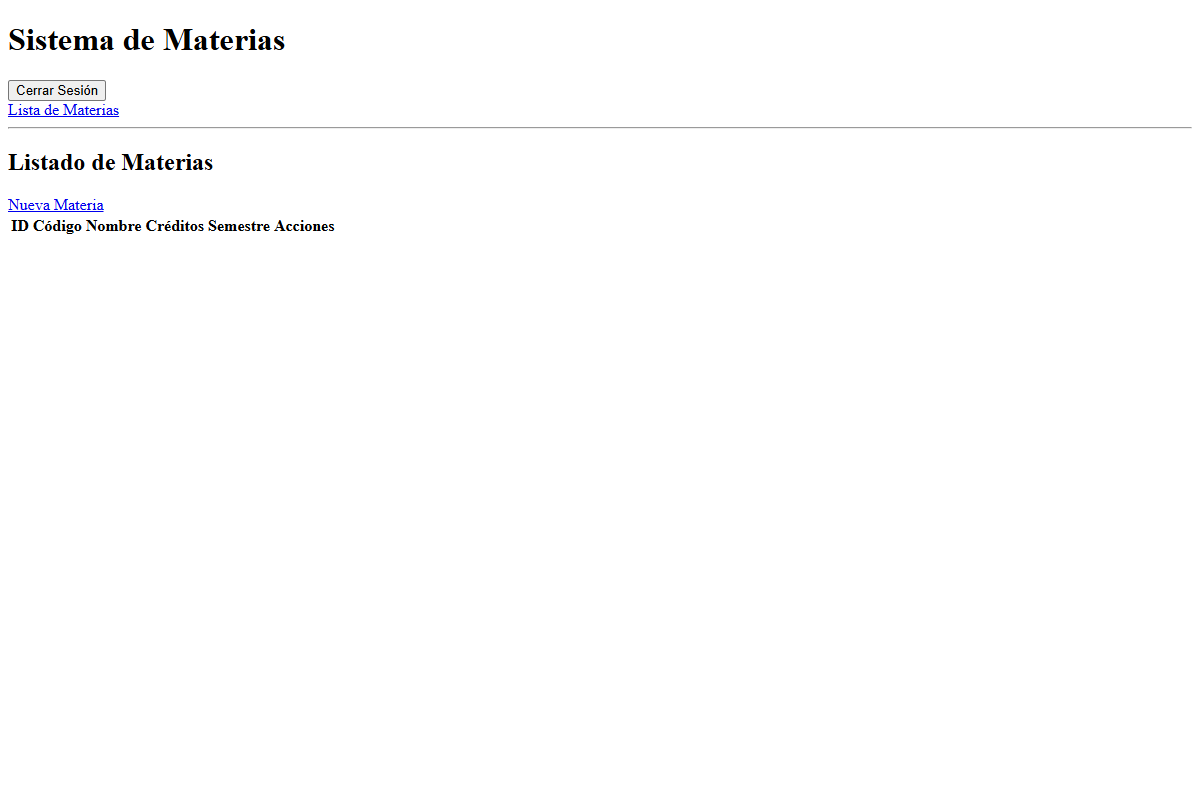
\includegraphics[width=0.8\textwidth]{capturas/05-eliminacion-logica.png}
  \caption{CRUD: Reflejo en tabla tras eliminación lógica.}
\end{figure}

\section{Requisitos Implementados}

\subsection{Arquitectura y Despliegue con Docker}
El repositorio incluye un archivo \texttt{docker-compose.yml} que configura y levanta tanto el contenedor web (PHP 8.3 y Apache) como el de la base de datos (PostgreSQL 15). Se crearon scripts en la carpeta \texttt{db/} (\texttt{schema.sql} y \texttt{seed.sql}) que inicializan automáticamente el esquema de datos y el usuario semilla con contraseña hasheada, permitiendo que la aplicación se levante con el único comando \texttt{docker compose up -d --build}.

\subsection{Patrón de Diseño MVC y Capas}
El sistema está diseñado bajo el patrón Modelo-Vista-Controlador y separa las responsabilidades de forma estricta:
\begin{itemize}
    \item \textbf{Controlador:} Recibe las peticiones HTTP, verifica los tokens CSRF y gestiona las sesiones (\texttt{MateriaController.php}, \texttt{AuthController.php}).
    \item \textbf{Servicio:} Lógica central que valida rangos, longitudes y unicidad de la información (\texttt{MateriaService.php}).
    \item \textbf{Repositorio (DAO):} Única capa con acceso directo a la base de datos mediante extensiones PDO, aislando las sentencias SQL (\texttt{MateriaRepository.php}).
\end{itemize}

\subsection{Seguridad OWASP Top 10}
Se han aplicado rigurosas medidas defensivas exigidas en la rúbrica:
\begin{itemize}
    \item \textbf{Inyección SQL:} Totalmente mitigada en la capa Repositorio al prohibirse la concatenación de datos del usuario, utilizando el formato paramétrico seguro de PDO (\texttt{:codigo}, \texttt{:nombre}, etc.).
    \item \textbf{Cross-Site Scripting (XSS):} Todo el flujo de salida dinámico que interactúa con las vistas HTML es sistemáticamente escapado usando \texttt{htmlspecialchars(..., ENT\_QUOTES, 'UTF-8')}.
    \item \textbf{CSRF:} Cada formulario originado por el método POST es validado en el servidor contra un token secreto y aleatorio (\texttt{random\_bytes(32)}) persistido en sesión. La comprobación se ejecuta en tiempo constante vía \texttt{hash\_equals}.
    \item \textbf{Cabeceras HTTP de Defensa:} Se emitieron las directivas de protección globales: \texttt{Strict-Transport-Security}, \texttt{X-Frame-Options: DENY}, \texttt{X-Content-Type-Options: nosniff} y un \texttt{Content-Security-Policy} básico restrictivo.
\end{itemize}

\subsection{Autenticación, Hashes y Sesiones}
El usuario semilla `admin` se crea con la clave `Admin*2026` protegida bajo algoritmo \textbf{BCrypt} directamente en la base de datos. La gestión de sesiones rechaza cualquier petición a una ruta de la aplicación (distinta al login) con un código HTTP 302 hacia `/login`. Las cookies de sesión operan bajo las banderas de seguridad \texttt{HttpOnly=true} y \texttt{SameSite=Strict}.

\section{Decisiones Técnicas}
Conforme a los requerimientos, las decisiones documentadas en la carpeta docs justifican la separación por capas (evitar código espagueti y mejorar testabilidad), la implementación rigurosa de PDO (frente a librerías inseguras o funciones arcaicas como \texttt{mysql\_query}) y las múltiples validaciones duales (tanto atributos HTML5 requeridos en cliente como rechazos controlados 422 en el backend).

\end{document}
